\documentclass{mcm}
\mcmsetup{CTeX = false,
    tcn = {16926},  %% your team control number
    sheet = true,
    titleinsheet = True,
    keywordsinsheet = true,
    titlepage = false,
    abstract = false}

\usepackage{newtxtext}%\usepackage{palatino}
\usepackage{comment}
\usepackage{lipsum}
\hypersetup{
    colorlinks=false,
    linkcolor=blue,
    filecolor=blue,
    urlcolor=blue,
    citecolor=cyan,
}
\usepackage{color}
\usepackage{float}
\numberwithin{figure}{section}
\numberwithin{table}{section}
\numberwithin{equation}{section}
\usepackage{enumerate}
\usepackage{placeins}
\usepackage[figuresright]{rotating}
\usepackage[final]{pdfpages}
\usepackage[
    backend=bibtex,
    style=numeric-verb,
]{biblatex}
\usepackage{babel}
\usepackage{changepage}
\usepackage{caption}
\usepackage{textcomp}
\usepackage{enumitem}
\usepackage{siunitx}
\usepackage{tabularx}
\usepackage{booktabs}
\usepackage{blindtext}
\usepackage{capt-of}
\usepackage{algorithm}
\usepackage{algorithmicx}
\usepackage{algpseudocodex}
\usepackage{tocloft}
\usepackage{wrapfig}

\graphicspath{{../../res/img/}{../../res/graphs/}}

\addbibresource{main.bib}


\title{Title}

\begin{document}

    \begin{abstract}
        Exec Summary

        \begin{keywords}
            Keywords, More Keywords
        \end{keywords}

    \end{abstract}

    \maketitle
    \tableofcontents
    \newpage


    \section{Q1: The Road Ahead}
    \graphicspath{{../../res/img/}{../../res/graphs/}}

\subsection{Defining the Problem}
In Problem 1, we were tasked with producing a short-term predictive model for e-bike sales.
More specifically, we were asked to develop projections for total sales volume 2 and 5 years into the future respectively.

This is a time-series forecast problem, where we predict a single variable - e-bike sales - based on a single input - time.
We will take a general approach of regressing particular equations against the existing data.
Multiple types of equations will be used and the most promising model will be chosen.

\subsection{Assumptions}
\noindent\textbf{Assumption 1}: There will be \underline{no major legislative changes}, governmental campaigns and/or ‘black swan’ (i.e., highly unpredictable and consequential) world events that significantly impact the market for e-bikes within the next five years.

\vspace{-6pt}
\noindent\textbf{Justification}: in practice, it is impossible to account for rare or extreme events within the constraints of a mathematical model; the implications of such events cannot be predicted with accuracy.

\noindent\textbf{Assumption 2}: The market for e-bikes in the European Union behaves comparably to that of the United Kingdom; therefore, \underline{British and European sales can be considered to be in direct linear} \underline{proportion}.

\vspace{-6pt}
\noindent\textbf{Justifications}: \\
\vspace{-24pt}
\begin{adjustwidth}{24pt}{0pt}
    \noindent\textbf{a)} Of the data provided for European sales, several figures appear to include sales made in the UK (CITE EBICYCLES.COM). Therefore, UK consumer behaviour is partially accounted for even within the larger dataset. \\
    \noindent\textbf{b)} E-bicycles have only begun gaining traction as a mode of transport in relatively recent years; as a result, UK-specific consumption data is largely unavailable to the public. \\
    \noindent\textbf{c)} To a large extent, the UK and EU follow similar urban planning practices that include pedestrian walkability and bicycle access.
    In other terms, city layouts support the practical use of e-bikes.
    For this reason, population-scaled EU predictions can be considered appropriate substitutes for UK-specific predictions.
    By contrast, most American cities use car-centric design, frequently involving longer commute distances and poor bike access.
    This renders the United States hostile to the adoption of e-bikes in a way that the EU and UK are not.
    For this reason, we chose to exclude the US from our analysis, instead focusing on the UK and EU.
\end{adjustwidth}

%\noindent\textbf{Assumption 3}: Statement
%
%\vspace{-6pt}
%\textbf{Justification}: blah blah

\subsection{Variables}
See table 1.1:
\begin{table}[h!]
    \centering
    \begin{tabular}{cc}
        \toprule
        Variable & Definition      \\
        \midrule
        $y_i$      & (actual) e-bike sales in year $i$     \\
        $\hat{y_i}$      & predicted e-bike sales in year $i$     \\
        \bottomrule
    \end{tabular}
    \caption{Variables in the Model}
    \label{tab:q1_vars}
\end{table}

\subsection{Models}

\subsubsection*{Linear}
A linear regression is performed first due to its simplicity and ability to help pick more complex models.

Linear regression is an approach used to model a linear relationship between an independent variable $x$ and a dependent variable $y$ by finding the slope of the trend and initial value ($y$ when $x$ is 0).
It is used to represent existing data and predict future values; linear models are used both for interpolation and extrapolation.
In this case, the model will be fit to existing data and used to predict future sales of e-bikes.
A linear growth function takes the general form of~\eqref{eq:lr}:
%
\begin{equation}
    f(x) = \alpha x + \beta
    \label{eq:lr}
\end{equation}
%
\noindent where $\alpha$ is the coefficient, or growth rate; and $\beta$ is the y-intercept, or initial value.
The values of $\alpha$ and $\beta$ are ``optimized'' using an algorithm to model a given dataset with the minimum ``error''.

One of the most common and simplest methods used to calculate the coefficient and intercept of the regression line is the Ordinary Least Square (OLS) \textit{optimization} method.
In short, OLS minimizes the Square-Error for each point against a given linear function by adjusting the function\textquotesingle s parameters, which in the end produces optimal parameters for a equation in the form of a linear line of best fit.

The Square-\textit{Error} function, which is what OLS \textit{optimizes}, is simply a summation of the squares of the difference between actual values and predicted values, over all data points~\eqref{eq:ls}:

\begin{equation}
    E = \sum{(y - \hat{y})^2}
    \label{eq:ls}
\end{equation}

Because the predicted values $\hat{y}$ for a linear model is modelled as $\alpha x + \beta$, the Square-Error function for a linear model can be more specific~\eqref{eq:ls_lr}:

\begin{equation}
    E = \sum{(y - (\alpha x + \beta))^2}
    \label{eq:ls_lr}
\end{equation}

OLS calculates the values of $\alpha$ and $\beta$ which minimize $S$ in the summation above.
Unlike the generic differential method described above, OLS is specialized for linear functions and can calculate the optimal parameters in one stop, using summation ratios.
The coefficient $\alpha$, or the linear trend of the dataset can be calculated with~\eqref{eq:lr_coef}:

\begin{equation}
    \alpha = \frac{n \sum x_i y_i - \sum x_i \sum y_i }{n \sum x^2_i - (\sum x_i)^2}
    \label{eq:lr_coef}
\end{equation}

\noindent where $n$ is the number of data points.

After calculating the slope of the trend, the intercept $\beta$, is calculated by~\eqref{eq:lr_intc}:
%
\begin{equation}
    \beta = \bar y - \alpha \bar x
    \label{eq:lr_intc}
\end{equation}

OLS was applied to the given data set to obtain the coefficient $\alpha$ and the y-intercept $\beta$ - $222.6$ and $446810$, respectively - which corresponds to the following linear equation:
%
\begin{equation}
    \hat y_i = 222.6 i - 446810
    \label{eq:ebike_lr}
\end{equation}
%
\noindent where $i$ is the year.

Linear regression is useful in relation to the problem as it is simple to interpret and portray, allowing the prediction of data to be accurate during interpolation.
However, if the data to be predicted is outside the range, i.e.\ predicting future e-bike sales, extrapolation may be inaccurate due to a false assumption of the trend.
Furthermore, if the variables plotted provide a non-linear relationship, a linear regression line may inaccurately represent and predict values, which is the case in the data provided.
Statistical error of the linear regression model against existing data shows a good but not perfect accuracy (Table~\ref{tab:ebike_lr_err}).

\begin{table}[h]
    \begin{minipage}{0.7\linewidth}
        \centering
        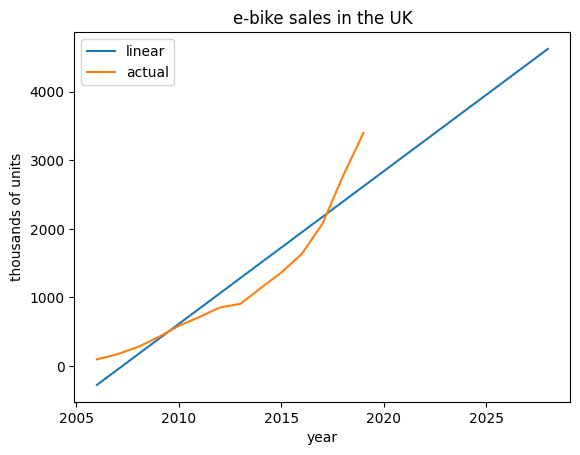
\includegraphics[width=\textwidth]{linear}%
        \captionof{figure}{Regressed Linear Model}
        \label{fig:ebike_lr}
    \end{minipage}%
    \begin{minipage}{0.3\linewidth}
        \centering
        \begin{tabular}{ll}
            \toprule
            Metric               & Value  \\
            \midrule
            MSE                  & 108671 \\
            RMSE                 & 329.65 \\
            MAE                  & 268.82 \\
            PCC                  & 0.9386 \\
            R\textsuperscript{2} & 0.8810 \\
            CVAR                 & 867138 \\
            \bottomrule
        \end{tabular}
        \vspace{8pt}
        \caption{Linear Model Statistics}
        \label{tab:ebike_lr_err}
    \end{minipage}
\end{table}


\subsubsection*{Exponential}

The second approach decided upon was exponential regression, which models the non-linear relationship between an independent variable $x$ and dependent variable $y$, where the rate of change of $y$ with respect to $x$ at a given point is proportional to the quantity itself.
This choice was made based on visual indicators of the data given\textquotesingle s trend, where the line graph exhibited a possible exponential curve.
Exponential growth functions take the general form of~\eqref{eq:exp}:
%
\begin{equation}
    f(x) = \alpha^x
    \label{eq:exp}
\end{equation}
%
\noindent where $\alpha$ is the exponential growth factor.

However, in order to fit such a model to arbitrary (non-normalized) values, two additional parameters have to be added to allow for displacement translations of the function on both axis. This gives:
%
\begin{equation}
    f(x) = \beta (\alpha)^{x + a} + b
    \label{eq:exp2}
\end{equation}
%
\noindent where $a$ and $b$ allows for offsets in the x and y axis, respectively.

An optimization can be made here - the equation can be rearranged to only have 3 parameters yet still be able to fit to any scale and offset of values:
%
\begin{equation}
    f(x) = B^{b (x + a)} + c
    \label{eq:exp3}
\end{equation}
%
\noindent where $B$, the base, can be any positive constant, and the function is parameterized by $a$, $b$, and $c$.

$a$ and $b$ performs a linear transformation on the input, while $c$ performs a translation on the output.
The equation in this form expresses in the relationship in purely in terms of translations.
This reduction in parameters allows for a higher efficiency when regressing the function to the dataset programmatically.
In the actual regression, 2 was used for the value of $B$.

Unlike linear regression, trying to calculate optimal parameters to an exponential model would technically require calculus concepts such as partial derivatives.
However, a programmatic approach was taken, and the function was ``blindly'' (without accounting for its algebraic structure) regressed using gradient descent (Alg.~\ref{alg:grad}) from derivative estimates.
The \verb|curve_fit()| optimizer from the Python SciPy library can blindly optimize any non-linear function to a dataset.
It is able to optimize unknown functions by performing gradient estimates~\eqref{eq:grad} of the error function with respect to the parameters using the basic definition of the derivative (at a given point, $x$):
%
\begin{equation}
    G = \frac{\Delta f(x)}{\Delta x} = \frac{f(x + \Delta x) - f(x)}{\Delta x}
    \label{eq:grad}
\end{equation}
%
\noindent where $G$ is the gradient of function $f$ at point $x$.
$\Delta x$ is set to a very small value to increase accuracy for sensitive functions.

After being able to calculate gradients of the error function at any point of the model function, a gradient descent algorithm~(\ref{alg:grad}) can be deployed to iteratively minimize the error function.
The parameters are adjusted based the gradients of the error function:
%
\begin{equation}
    \beta_j \longleftarrow \beta_j - \alpha \frac{E(x, \beta + \Delta \beta_j) - E(x, \beta)}{\Delta \beta_j}
\end{equation}
%
\noindent where parameter $\beta_j$ is adjusted based the error function $E$\textquotesingle s gradient - the parameter changes in to the opposite direction of the gradient in order to find the minimum of the error function.
$\alpha$, the learning rate, is usually a very small value to prevent the parameters from changing too much at once.

\begin{algorithm}
    \caption{Gradient Descent}
    \label{alg:grad}
    \begin{algorithmic}
        \Repeat
            \State $\epsilon \gets E(f(x, \mathbf{\beta}))$  \Comment{E is the error function}
            \State $\gamma \gets \frac{\Delta E(f(x, \mathbf{\beta}))}{\Delta \mathbf{\beta}}$  \Comment{calculate current gradient}
            \State $\mathbf{\beta} \gets \mathbf{\beta} - \alpha \gamma$  \Comment{$\alpha$ is the learning rate}
        \Until{$\epsilon$ \text{ is sufficiently small}}  \Comment{$\epsilon$ is the error or residuals}
        \State \Return $\mathbf{\beta}$ \text{ as the optimal parameters}
    \end{algorithmic}
\end{algorithm}


The SciPy curve fit optimizer was applied to the given data to obtain the following function~\ref{eq:co2_exp}.
The exponential model was graphed alongside the actual values and the linear model for comparison in Figure~\ref{fig:ebike_exp}.
%
\begin{equation}
    \hat C_i = 2^{0.023381 (i - 1707.690634)} + 256.024002
    \label{eq:co2_exp}
\end{equation}

\begin{table}[h]
    \begin{minipage}{0.7\linewidth}
        \centering
        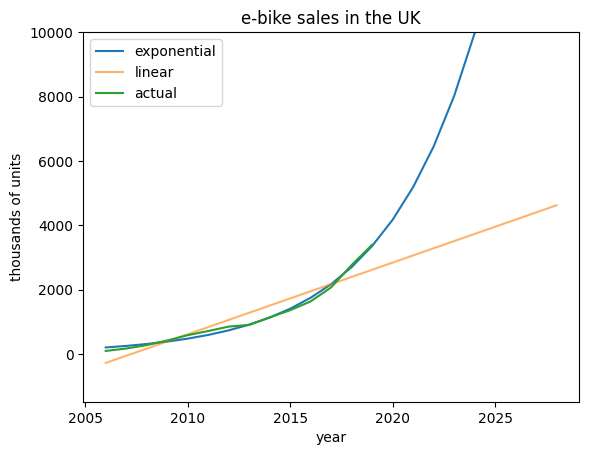
\includegraphics[width=\textwidth]{exponential}%
        \captionof{figure}{Regressed Exponential Model}
        \label{fig:ebike_exp}
    \end{minipage}%
    \begin{minipage}{0.3\linewidth}
        \centering
        \begin{tabular}{ll}
            \toprule
            Metric               & Value   \\
            \midrule
            MSE                  & 0.48061 \\
            RMSE                 & 0.69326 \\
            MAE                  & 0.56981 \\
            PCC                  & 0.99973 \\
            R\textsuperscript{2} & 0.99945 \\
            CVAR                 & 890.45  \\
            \bottomrule
        \end{tabular}
        \vspace{8pt}
        \caption{Exponential Model Statistics}
        \label{tab:ebike_exp_err}
    \end{minipage}
\end{table}

Visually, the exponential function better aligns with the actual values; the predicted values also seem to fit with the general trend, and this is confirmed by extremely good error metrics, as show in Table~\ref{tab:ebike_exp_err}.
An advantage of exponential regression as a predictive model is that it provides high quality forecasts, which increase the accuracy of predicted values during interpolation.
However, a key drawback is that a large data set is necessary to carry this method out, as a reasonable amount of continuity is needed to accurately predict future values, especially during extrapolation.

Initially, our team planned on only using a linear regression model, even though visually the data trend and the model did not match. We came to the conclusion to also implement an exponential model to provide a point of comparison, and to examine whether our initial visual cue did indeed follow an exponential trend.

To carry this out, we found that Python and Jupyter were the better choice over Excel, as we were able to have a higher degree of control over the parameters and values outputted by the functions. Additionally, the error metric functions we defined could be use for the next problems, which would increase our efficiency as less code would need to be re-written.

\subsubsection*{Tilted Sigmoid}

See~\ref{fig:tilted}

\begin{table}[h]
    \begin{minipage}{0.7\linewidth}
        \centering
        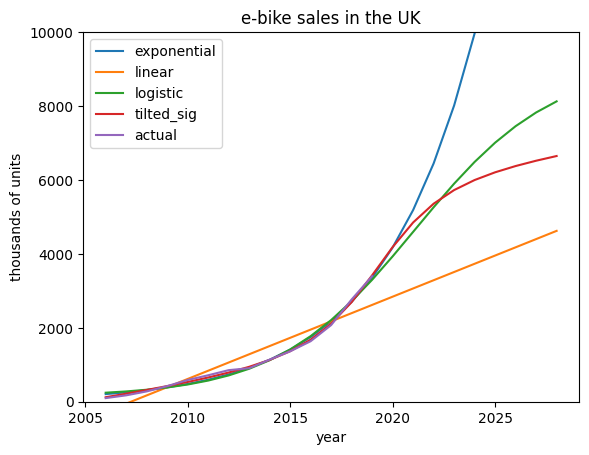
\includegraphics[width=\textwidth]{titled-sigmoid}%
        \captionof{figure}{Regressed Tilted Sigmoid Model}
        \label{fig:tilted}
    \end{minipage}%
    \begin{minipage}{0.3\linewidth}
        \centering
        \begin{tabular}{ll}
            \toprule
            Metric               & Value   \\
            \midrule
            MSE                  & 0.49061 \\
            RMSE                 & 0.71326 \\
            MAE                  & 0.52381 \\
            PCC                  & 0.99973 \\
            R\textsuperscript{2} & 0.99945 \\
            CVAR                 & 895.45  \\
            \bottomrule
        \end{tabular}
        \vspace{8pt}
        \caption{Tilted Sigmoid Statistics}
        \label{tab:t}
    \end{minipage}
\end{table}


    \section{Q2: Shifting Gears}
    \subsection{Defining the Problem}
For problem 2, we were instructed to identify underlying factors for the growth models depicted in problem 1, and determine the most impacting factors by constructing a mathematical model.

\subsubsection*{Limitations}

Naturally, data analysis methods can only best prove correlation while lack at proving cause-and-effect relationships.
We identified possibly correlated factors (datasets) and computed relecant bivariate statistics to measure how well an independent factor can predict and possible affect the sale of e-bikes.


\subsection{The Model}
Our approach to this problem first involved selecting the most significant factors affecting e-bike sales growth. Our final list included the main factors provided in the question, as well as an additional one chosen by our team. Each factor was then quantified as shown below:


\begin{table}[h!]
    \centering
    \begin{tabular}{cc}
        \toprule
        Factor & Quantified Measure      \\
        \midrule
        Health   & Death by cardiovascular illness per 100000     \\
        Gas Prices (Diesel) & E-Bikes sold (1000s of units)     \\
        Environmental Perception & Percentage of survey respondents selecting Environment\\
        Disposable Income & Per capita in GBP\\
        \bottomrule
    \end{tabular}
    \caption{Factors}
    \label{tab:factors}
\end{table}

Other ``factors'' that logically do not directly affect the sale of e-bikes are still analyzed for relevant correlations:

\begin{table}[h!]
    \centering
    \begin{tabular}{cc}
        \toprule
        Factor & Quantified Measure      \\
        \midrule
        Emissions   & CO\textsubscript{2} emissions per capita    \\
        EV Sales & Sales of Battery-EVs and Hybrid-EVs     \\
        Population & total population \\
        \bottomrule
    \end{tabular}
    \caption{Other ``Factors''}
    \label{tab:factors2}
\end{table}


To determine the most impacting factor on bike sales, we decided implement the predictive model ARIMA, which we would construct and apply to each factor above.
The model would then be used to predict future values, which can then be used in conjunction with E-Bike sales to examine their correlation. Error metrics are then
to be evaluated for each correlation; the most accurate model would be deemed as the most significant factor.

As for the specifics of ARIMA, this model is widely used in datasets that demonstrate non-stationarity, where the series' statistical properties such as
mean, variance and autocorrelation change over time. ARIMA assumes the input data to
be stationary, so any non-stationary data has to be made stationary through a reversible
process. Usually, the transformation involves finding the general trend with methods such as
regression and then using diffencing to remove the trend from the dataset. With the trend
eliminated, an ARIMA model can then be constructed and its optimal parameters found.

The parameters are denoted in the form ARIMA(p, d, q) where $p$ is the
number of Auto-Regressive (AR) terms, $d$ is the orders of differencing, and $q$ is the number
of Moving Average (MA) terms.

The functions AR(p) and MA(q) are defined below as:


\begin{tabular}{|*2{p{.45\textwidth}|}}
    \hline
    AR(p):                       & MA(q):                   \\
    \quad ${\phi (B) X_t = w_t}$ & ${X_t = \theta (B) w_t}$ \\[\baselineskip]
    Where
    \begin{itemize}[nosep]
        \item ${\phi (B)}$ = Autoregressive operator
        \item ${X_t}$ = Inverse operator
        \item ${w_t}$ = White noise
    \end{itemize}
    &
    Where
    \begin{itemize}[nosep]
        \item ${\theta (B)}$ = Moving average operator
        \item ${X_t}$ = Inverse operator
        \item ${w_t}$ = White noise
    \end{itemize}
    \\
    \hline
\end{tabular}

Before tuning the parameters p and q, the number of differencing required to make the
data stationary must be found out. To evaluate whether the current dataset is stationary, an
Augmented Dickey-Fuller (ADF) test was performed.
ADF tests expand on the original Dickey-Fuller test by including higher-order autoregressive
processes to form the equation:


\begin{equation}
    \Delta y_{t}=\alpha +\beta t+\gamma y_{t-1}+\delta _{1}\Delta y_{t-1}+\cdots +\delta _{p-1}\Delta y_{t-p+1}+\varepsilon _{t}
\end{equation}
%
where
${y_{t}}$ is the value of the time series at time t,
${\alpha}$ is a constant,
${\beta}$ is the coefficient of the trend, and
$p$ is the lag order of the autoregressive process.

If data is stationary, then ACF (autocorrelation functions) and PACF (partial autocorrelation functions) can be used.
AFC and PAFC functions are measures of correlation between past
and present data, and indicate which past data values are most useful in predicting future
ones. The results of these functions are then used to select the most optimal parameters for
p and q.

The ADF test, ACF, and PACF plots were applied onto each factor; the results can be viewed in the bibliography.

\subsection{Results}

We hypothesised that seven identified factors were likely to influence the market for e-bikes over the next five years.
Each factor has its values normalized between 0 and 1, so that the calculated bivariate statistics are comparable.
This is because we do not care about the magnitudes of these figures, since they are completely irrelevant and independent; we only care about the trend and patterns in the data.

Bivariate analysis was performed on each factor against the sale of e-bikes, and the results are summarized in table~\ref{tab:factor_bivar}:

\begin{table}[h!]
    \centering
    \caption{Bivariate Statistics of each Factor}
    \begin{tabular}{cccc}
        \toprule
        Factor & PMCC & R\textsuperscript{2} & Covariance      \\
        \midrule
        Emissions   & -0.900 & 0.811 & -425    \\
        EV Sales & 0.902 & 0.814 & 359     \\
        Population & 0.906 & 0.821 & 440 \\
        Gas Price & 0.363 & 0.132 & 171 \\
        Environmental Perception & 0.967 & 0.936 & 443 \\
        Disppsable Income & 0.324 & 0.105 & -386 \\
        Death Rate & -0.899 & 0.641 & -385 \\
        \bottomrule
    \end{tabular}
    \label{tab:factor_bivar}
\end{table}

Through this correlation analysis, we determined that the three most significant factors affecting e-bike usage were, in order, environmental perception, population and electric vehicle (EV) sales.

We defined ``environmental perception'' as a metric for societal awareness and concern about climate-related issues. We quantified this through results obtained in the UK YouGov poll from 2011-22. This revealed that heightening environmental perception coincided with an increase in e-bike usage. More specifically, there was a high r\textsuperscript{2} value of approximately 0.936, indicating a strong correlation. This is corroborated by real-world social phenomena. In recent years, increasing media coverage, highly publicised climate summits and more prolific environmental education, among other contributing factors, have brought the climate crisis to the forefront of the public consciousness. Although it would be premature to definitively conclude that changing attitudes led to the increased adoption of e-bikes, it is likely that the changing social landscape motivated more consumers to opt for more environmentally friendly modes of transport. E-bikes are far less polluting than conventional, fossil-fuel driven vehicles, and therefore likely benefitted from this mentality shift.

As expected, increased demand for e-bikes also correlated with population growth (r\textsuperscript{2} = 0.821). The reasons for this are likely more explicit: a larger population requires greater quantities of transport. E-bikes likely benefitted from this greater general trend, resulting in increases in usage over several years of population growth.

Increased EV sales also showed a strong correlation with e-bike sales (r\textsuperscript{2} = 0.813). Rather than a simple causation, this was likely due to a more nuanced interdependence. As EV usage grew, public awareness and acceptance of electrical mobility grew with it. This trendiness in turn led to greater demand for e-bikes. The same effect may have applied in the opposite direction, whereby increased e-bike use resulted in greater demand for electric vehicles in general. It is therefore impossible to determine whether more EV use truly led to the increase in e-bike sales or whether more intricate behavioural factors were at play.

Besides the three principal factors, we found that two further variables were moderately correlated with increased e-bike use: carbon dioxide emissions per capita and the death rate from cardiovascular disease.

There was a moderate negative correlation between emissions and e-bike usage (Pearson correlation coefficient = -0.900; r\textsuperscript{2} = 0.811). Realistically, it is unlikely that e-bike usage caused a drastic decrease in carbon dioxide emissions, due to the fact that it accounts for a relatively small proportion of the transport sector. Simply put, this correlation may result from the fact that both variables increased significantly over time, albeit relatively independently. Alternatively, increased emissions may link with greater environmental awareness, discussed above.

Furthermore, we discovered an unexpected weak-to-moderate positive correlation between the death rate from cardiovascular illness and e-bike use (r\textsuperscript{2} = 0.641). This could potentially occur due to greater health awareness and resulting demand for exercise goods; however, given the relatively low correlation strength, it is far more likely to be coincidental.

The two factors that have little to no correlation to e-bike sales are gas prices and disposable income. Gas prices have an r\textsuperscript{2} value of 0.132, meaning there is a weak correlation between rising gas prices and e-bike sales over time. This is due to existing infrastructure being built up on gas, oil and other non-renewable resources, meaning that consumers rarely switch to other substitutes such as e-bikes, despite large increases in oil prices (as occurred at the outbreak of the war in Ukraine). Regardless, a covariance of 171 highlights that there is a positive relationship, making e-bikes a more attractive option for consumers as rising gas prices increase the costs of driving a car.

Disposable income has an r\textsuperscript{2} value of 0.105, meaning that there is insignificant correlation between an individual\textquotesingle s disposable income and e-bike sales. This is due to a large amount of other desired goods by consumers, causing them choose other goods instead of e-bikes, due to personal preference. However, factors such as social influence and cultural attitudes can influence individual consumer choice, unrelated to disposable income.

Recent sociological research provides experimental evidence for a quantified tipping point in social convention. That is, once a sufficiently large minority embraces a new technology or consensus, the rest of society is incentivised to follow. Centola et al. define this tipping point at 25\% of the population. This provides a useful metric for societal receptiveness towards e-bikes as a mode of transport. We chose the UK National Travel Attitudes Study (NTAS) 2021 in order to quantify social preferences. Only 4\% of all respondents owned or had regular use of an e-bike. Out of those who had never used an e-bike, 35\% indicated that they would be interested in riding an e-bike if [they] had the chance to do so.  This is significantly greater than the 25\% tipping point, suggesting that the British public is sufficiently supportive of e-bikes – at least in principle – for them to become widely accepted in the future. However, at present, this does not translate to effective demand; most respondents indicated a low likelihood of actually purchasing an e-bike, even with a variety of options for financing. This semi-quantitative analysis implies that the immediate future may be decisive; demand may be influenced to new heights, but an alternative, more pessimistic outlook would suggest that sales may stagnate.


    \section{Q3: Off the Chain}
    \subsection{Defining the Problem}
Defining the Problem

\subsection{Assumptions}
\noindent\textbf{Assumption 1}: Statement
\textbf{Justification}: blah blah

\noindent\textbf{Assumption 2}: Statement
\textbf{Justification}: blah blah

\noindent\textbf{Assumption 3}: Statement
\textbf{Justification}: blah blah

\subsection{Variables}
See table 2.1:
\begin{table}[h!]
    \centering
    \begin{tabular}{cc}
        \toprule
        Variable & Definition      \\
        \midrule
        $x$      & description     \\
        $y$      & description     \\
        $z$      & description     \\
        \bottomrule
    \end{tabular}
    \caption{Variables in the Model}
    \label{tab:my_label}
\end{table}

\subsection{The Model}
Model

\subsection{Results}
Results

\subsection{Model Revision}
Model Revision

\subsection{Discussion}

\noindent\textbf{Strength 1}: asdf

\noindent\textbf{Strength 2}: asdf

\noindent\textbf{Weakness 1}: asdf

\subsection{Sensitivity Analysis}
Sensitivity Analysis

\subsection{Technical Computing}
Technical computing


\newpage


    \section{References}

    \subsection{Bibliography}
    \printbibliography

    \subsection{Program Code}
    \noindent Result data generated:
    \begin{verbatim}
    text data stuff

    \end{verbatim}

    \noindent Python program code:
    \begin{lstlisting}[language=Python,label={lst:code}]
        # pass

    \end{lstlisting}

\end{document}
